\subsection { 多级库存的优化}

    常见的多级库存优化管理的方法有两种:顺序排列法和DRP法。

\subsubsection { 一、顺序排列法}

    这方法遵循了基本路线。在单层级案例中所采用的方法在多层级案例中实施了两次——一次在他们库存驱动因素的基础上对DC 进行了补货,然后在基于它的库存驱动因素的基础上向RDC 进行补货。在这个案例中,DC 利用了终端客户需求和RDC 前置时间。RDC 的前置时间是十分明显的;它们仅仅是对供应商而言的。但是怎么为RDC 进行需求预测呢?一种方法是将需求建立在从DC 到RDC 的历史订单基础之上。另一种方法是简单地传递来自DC 终端客户的需求。正如我们所看到的那样,这两种方法都是有缺陷的。

    \begin{figure}[bcth]
        \begin{center}
            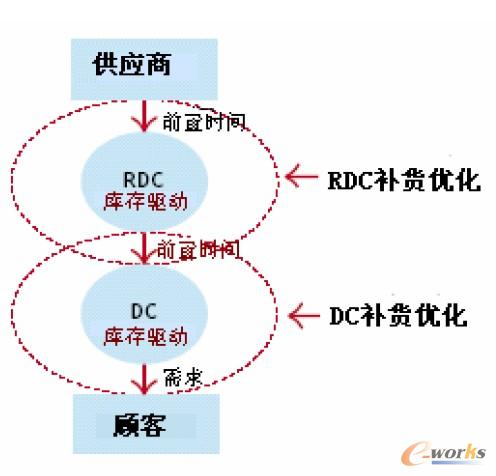
\includegraphics[scale=.6] {mlopt-1.jpg}
            \caption{顺序排列法} \label{fig:mlopt1}
        \end{center}
    \end{figure}

    图 \ref{fig:mlopt1} 说明了DC 和RDC 的补货方法,如前所述。这是一个顺序排列法,它将多级补货过程分成两个独立的阶段——一个阶段是为DC 补货,另一个阶段是为RDC 补货。但是这种方法带来了许多问题:

    \begin{enumerate}
        \item  缺乏需求链前向可视性

        当 DC 进行补货时,处于RDC 上游的供应商通常被遗忘。特别是DC 往往会忽视前置时间,当然除了来自RDC 的前置时间之外。而DC 一般也想当然地认为RDC 会在任何时间都能完全满足它的补货订单需求。最后,DC 对于RDC 的库存状况没有可视性。

        \item  缺乏需求链后向可视性

        当 RDC 进行补货时,通常会遗忘DC上游的客户。此外,RDC 对于DC 的库存状况货需求状况也没有可视性。

        \item  牛鞭效应带来的需求扭曲

        因为 RDC 和DC 有独立的需求预测(在基于他们各自直接的客户需求),牛鞭效应在RDC 和DC 之间造成了需求波动。这个结果导致RDC 不必要的库存。

        \item  整个网络成本难以评估

        当 RDC 或DC 的补货策略发生变化(如,通过改变可控库存驱动因素),新策略在另一级产生的隐含成本没有考虑进来。人们通常仅仅关注于对最近一级产生的影响。
    \end{enumerate}

\subsubsection { 二、配送需要计划法}

    配送需要计划(DRP)是材料供应计划(MRP)的拓展。制造商利用MRP 对零部件需求进行决策。用来制造产成品的零件或者部件是需求相关项目。正如MRP 那样,DRP 方法不管理生产组合不同阶段相关的需求,它对产品处于不同配送网络层级的需求进行管理。在某种意义上说,更高一层级中的产品需求取决于对相同产品低一级的需求。采用DRP 方法,DC 水平的需求预测首先被用来开拓整体产品需求。这些预测和安全库存需求、库存状态信息结合在一起,最终得出DC 的净需求。这是一种类似于MRP 综合图表的方法。通过弥补由RDC 到DC 前置时间产生的DC 净需求并且加总相应的时间周期,RDC 各阶段的时程化需求得到计算。RDC 利用这些上传的需求进行补货。DRP 方法也有些缺点。它首要的缺陷是上传需求和前置时间的非确定性。一个直接的结果是RDC 安全库存通常是在主观的方式下进行决策的。因为需求确定地上传至RDC,所以没有进行安全库存决策的严格性方法。这也是为什么使用这种补货方法的企业一般对RDC 安全库存量使用拇指规则;这种不科学的方法直接产生了多余的库存。由此,如果安全库存决策在一定程度上是不精确的,那也一点都不令人惊讶了。DRP 方法在制造领域中已经比较常用了,生产和运输成本通常也比库存成本更令人关注。正如顺序排列方法一样,DRP 不能拓展需求链前向的可视性,也缺乏对库存优化的整体网络性看法。

    特别需要指出的是,两层级的安全库存之间是没有任何联系的。因此,任何试图打破两层级之间的最佳平衡库存都是不可行的。

\subsubsection { 三、对顺序排列和DRP 方法的评价}

    顺序排列和 DRP 方法都会导致多余的库存,也没有对最终客户必要服务水平的改进。虽然每一层级可能获得合理的结果——来自它对整体问题的近视性看法——结果不一定是对整个网络最佳的解决方案。也就是说,DRC 和DC 的全部库存在追求最终客户服务目标方面没有达到最小化。

\subsubsection { 四、多层级网络中的牛鞭效应}

    对于牛鞭效应以及它扭曲需求信息已经谈过很多了。虽然牛鞭效应也可能在单层级解决方案中出现,但是它通常是企业所不能控制的。

    然而,在多层级网络中事实就不是这样了。在这些案例中,企业一定要考虑和管理牛鞭效应。牛鞭效应是在需求信号处理、订单计量、对价格波动和短缺博弈的反应过程中,由独立理性决策引起的。顺序排列方法通过在不同层级使用多独立需求预测而陷入了牛鞭效应之中。在低层级中订单计量引起层级之间额外的需求变化。最后,在顺序排列或DRP 方法中,缺乏需求供应链前向和后向的可视性能为实现客户服务目标而产生过多的库存积累。一个多层级网络提供正确测量牛鞭效应的机会,以此确定它的根源,减少或消除它对需求供应链绩效的影响。忽视这种机会也就意味着让牛鞭效应降低预测的准确性,增加库存,增加运作成本,降低客户服务水平。

\subsubsection { 五、真正的多层级方法}

    当一个有多层级网络的企业使用多层级方法管理库存时,主要的目的在于在所有的层级中最小化总库存,同时满足对最终客户的服务承诺。既使库存是主要的焦点,但是运输、仓储运作费用同样也在考虑之中,因为它们的成本因素也是优化的一部分。顺序排列和DRP方法将每个层级都看成是一个独立的问题,没有考虑到一个层级的库存可能对另一个层级可能产生较大的影响。采用多层级方法,需求预测和库存补货决策在单个优化过程中是在企业这个层面进行的。具体来说,真正的多层级方法应该是这样的:

    \begin{enumerate}
        \item  避免每个层级中的多头独立预测

        在 DC 的主要客户需求信号和其他信息驱动着所有层级的预测。真正的多层级方法消除了对于下游客户需求的依赖。

        \item  计算所有前置时间和前置时间的波动

        在每个层级上,补货决策计算了所有上游供应商而不仅仅是直接供应商的前置时间和前置时间的波动。

        \item  控制和管理牛鞭效应

        企业测算需求扭曲和确定可能采取的正确行动的根源。

        \item  实现需求链前向和后向的可视性

        每个层级利用其他层级库存位置的可视性——现有的、已定购尚未交货的、履行和延期交货的。在DC 层级,这意味着否定了对短缺博弈的任何需要。在RDC 层级,对DC 库存的可视性改进了需求的产生。

        \item  同步化订单策略

        将 DC 的订货周期与RDC 的运作实现同步化能减少RDC 和DC 之间的前置时间和前置时间波动。多层级模式能评估对不同同步化策略对两个层级的冲击。

        \item  提供差异化服务水平

        RDC 能为不同的DC 提供不同的服务水平(相同的产品)。一个多层级方法使之成为可能,因为企业控制一个产品在什么时间以什么方式进入或者离开RDC。

        \item  正确模拟一个层级替代性补货策略对另一个层级的交互式影响

        替代性策略包括不同补货周期、订单供应策略、服务水平目标和 SKU 层化。
    \end{enumerate}
